\prompt{Use Maximum Likelihood Estimation to fit the data given to a two-parameter Weibull distribution}


\begin{figure}[ht]
    \centering
    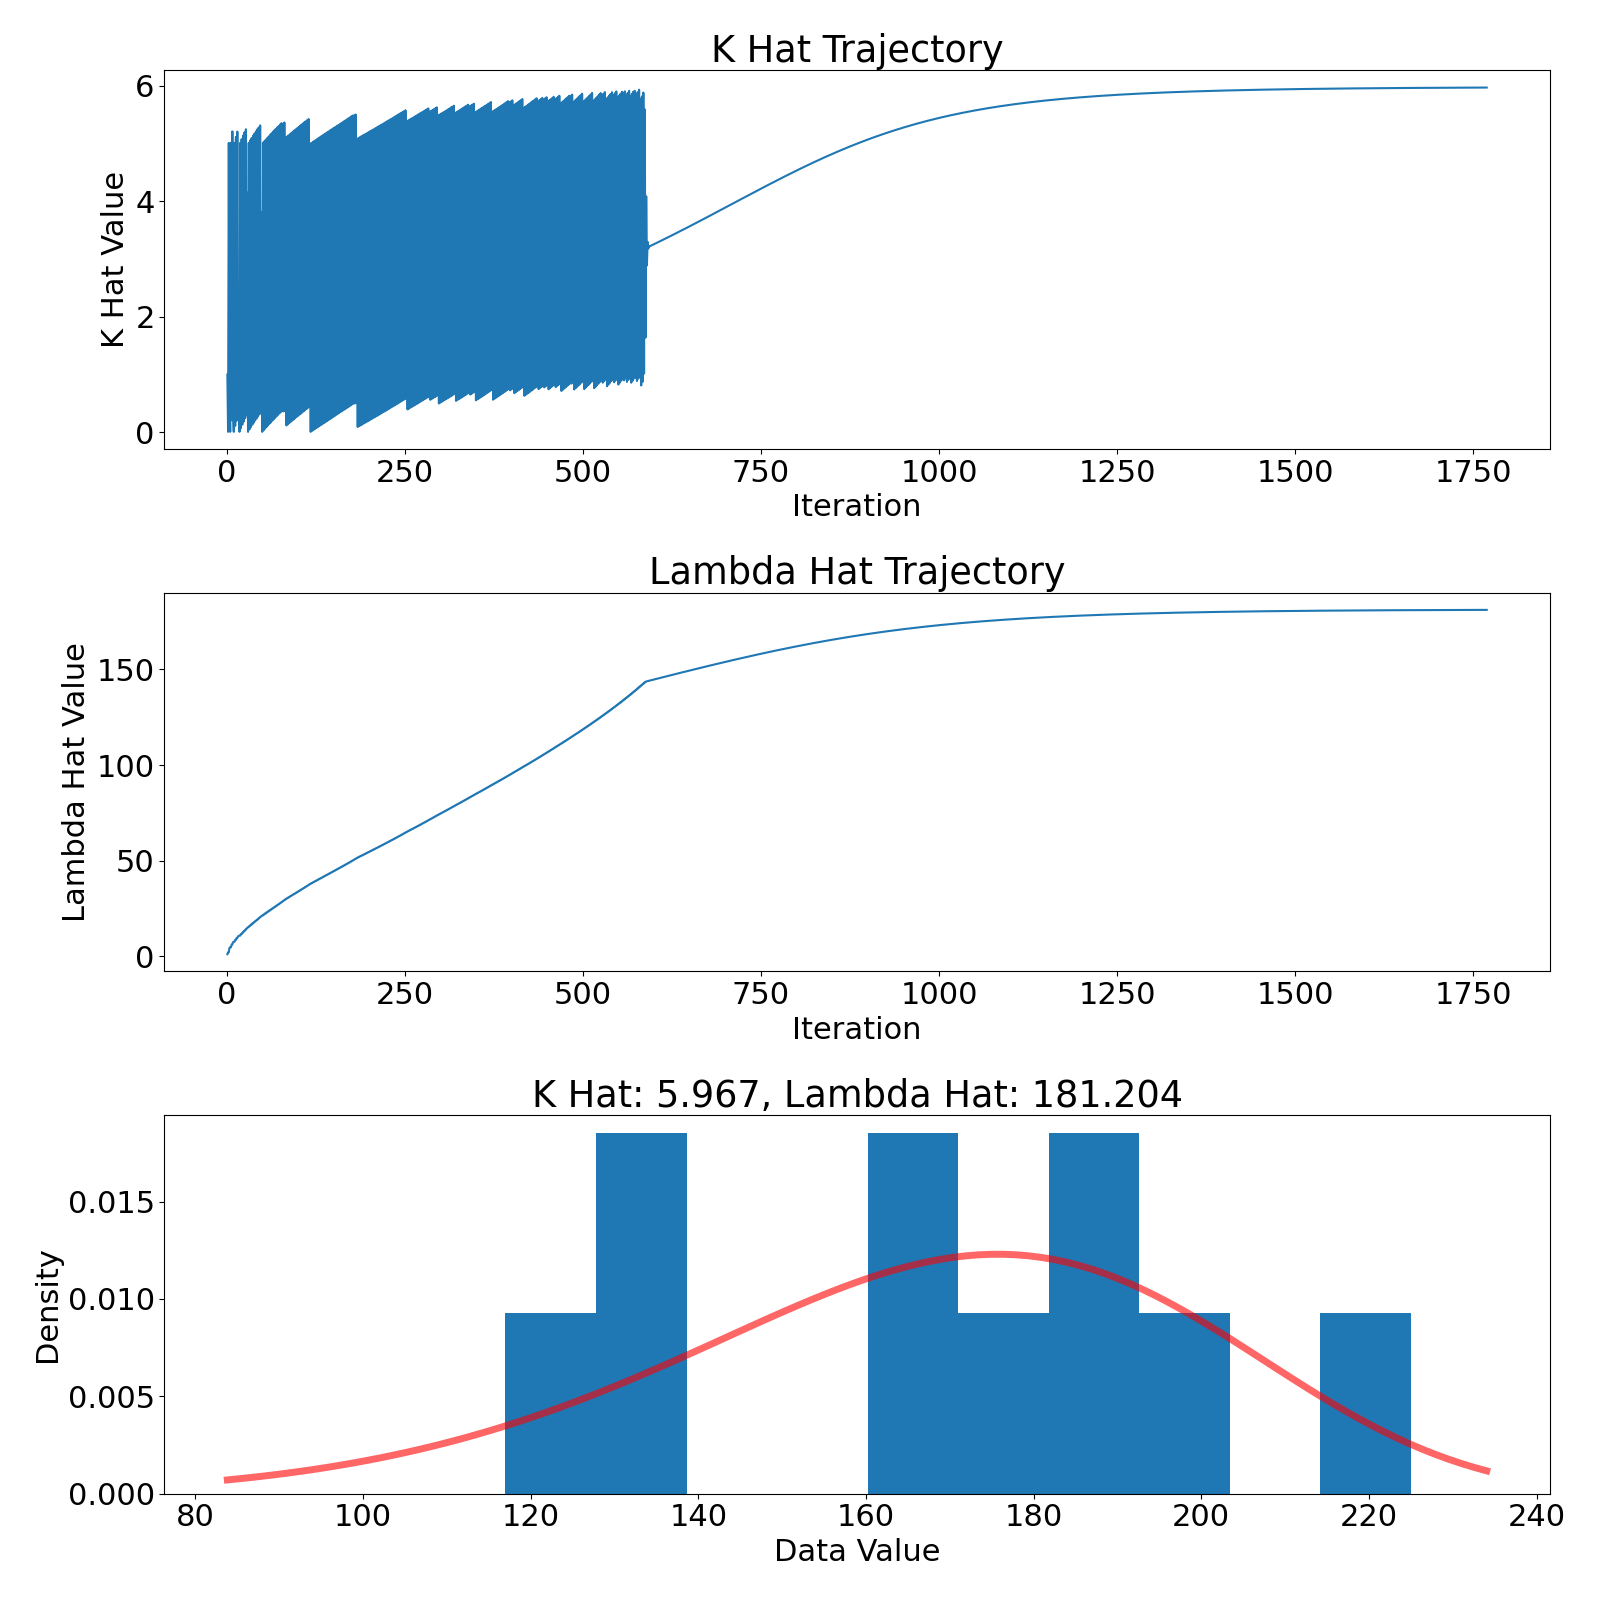
\includegraphics[width=0.5\textwidth]{figs/weibull_estimation.png}
    \caption{Weibull Parameter Estimation}
    \label{fig:Weibull_fit}
\end{figure}

The Weibull distribution proved harder to fit than the Cauchy.
Not only are there restrictions on the parameter space, but often as the optimization trajectory approached these limits, the gradient would explode and make the estimate unstable.
To alleviate this, I used gradient clipping to cap the L2 norm of the gradient to 10.
Without this I found the optimization to be unstable and unpredictable. 

I used Step-wise Gradient Descent as my algorithm because I did not want to compute the second derivatives.
However in retrospect, I could have saved myself a lot of time using the Newton-Raphson Method because the updates would have likely been more stable.

Figure \ref{fig:Weibull_fit} shows the trajectory of both parameter estimates as well as the final fit.
It took well over 1000 iterations to achieve a good fit, but it took a lot of experimentation to get this result.
I found that the decay rate had to be flattened substantially to $1-1e-10$ when initializing both parameters to $1.0$.
